\documentclass{article}
\usepackage[margin=1in]{geometry}
\usepackage{amsmath, amssymb, amsthm}
\usepackage{enumitem}

% colored links
\usepackage{hyperref}
\hypersetup{
    colorlinks=true,
    linkcolor=blue,
    filecolor=magenta,      
    urlcolor=blue,
    }




% Inputting Python code
\usepackage[dvipsnames]{xcolor}
\definecolor{textblue}{rgb}{.2,.2,.7}
\definecolor{textred}{rgb}{0.54,0,0}
\definecolor{textgreen}{rgb}{0,0.43,0}
\usepackage{upquote}
\usepackage{listings}
\lstset{
    language=Python, 
    tabsize=4,
    basicstyle={\ttfamily},
    keywordstyle=\color{textblue},
    commentstyle=\color{textgreen},
    stringstyle=\color{textred},
    frame=none,
    columns=fullflexible,
    keepspaces=true,
    showstringspaces=false,
    xleftmargin=-15mm, % manual adjustment, figure out permanent solution
}

%Creating algorithms
\usepackage{algorithm}
\usepackage[noend]{algpseudocode}

\usepackage{tcolorbox}
\tcbuselibrary{skins,hooks}
\usetikzlibrary{shadows}
\usepackage{lipsum}

%Images
\usepackage{graphicx}
    \usepackage{subcaption}
    \usepackage{float}
    % \usepackage[labelsep=period]{caption}

    
%Creating Figures
\usepackage{tikz}
\usetikzlibrary{calc, math, matrix, graphs, positioning}

%Formatting and Spacing
\setitemize[1]{noitemsep, parsep = 5pt, topsep = 5pt}
\setenumerate[1]{label = (\alph*), parsep = 1pt, topsep = 5pt}
\setlength\parindent{0pt}
\linespread{1.1}

% title
\title{\vspace{-1cm}CS 2051: Honors Discrete Mathematics \\Spring 2023 Homework 5 Supplement}
\author{Sarthak Mohanty }
\date{}

\begin{document}

\maketitle

\section*{Overview}
    \textbf{Note: This is a minimal working copy. It's missing a lot of context, and is only meant to help you get started with the homework early. I'll be updating it a lot more tomorrow with detailed instructions, more examples, and better formatting.}

    \vspace{2mm}
    Traditionally, computer software has been written for serial computation: instructions corresponding to a tasks are executed on one processing unit at a time. However, nowadays many computational tasks consist of many elementary operations, some of which had to be computed sequentially, while others could be computed in parallel. 

  % In a distributed computing or high performance computing class, one of the first things you learn is \textbf{Amdahl’s law}, which gives a quantitative measure of the speedup $S$ -- i.e., how much faster the task can be performed by using $n$ parallel processors:
  % $$S = \frac{1}{1 - p + \frac{p}{n}}.$$ Here, $p$ is the proportion of operations that can be performed in parallel.

  %   \vspace{2mm}
  %   However, it is not typically the case that we can classify operations simply as “parallel” or “sequential.” Instead, a task might consist of several sub-tasks, some of which need to be completed before others are started. 

  %   \vspace{2mm}
  %   To understand this problem, we first have to develop some mathematical foundations. This week in your 2050 lecture, you learnt about functions, and how they represent mappings between two sets. 
    

    \vspace{2mm}
    In this supplement, you learn about a generalized form of functions known as \textbf{relations}, and explore the connection between functions and relations. You'll learn about equivalence relations and partial orders. You'll also explore some of the applications of these concepts
  %   \vspace{2mm}
  %   Finally, we'll cover scheduling with multiple processors. You'll learn how to apply the theory of partial ordering through code. We'll cover topics such as \textbf{chains}, \textbf{antichains}, and \textbf{Dilworth's Lemma}.




\section*{Part 1: Relations and Graphs}

    % This week, you learned about functions. We (informally) defined them as a well-defined mapping between two sets. However, this leads us to two natural questions:
    % \begin{enumerate}[label = \arabic*.]
    %     \item 
    % \end{enumerate}
    
    We begin with (binary) relations, a mathematical representation for associating elements of sets.
    
    \vspace{3mm}
    \textbf{Definition} a \textit{relation} over sets $A, B$ is a subset of $A \times B$. The notation $a\mathcal{R}b$ or $a \sim b$ is often used to denote that $(a, b) \in \mathcal{R}$.
    
    \vspace{1.5mm}
    We denote relations by $\mathcal{R}$. We write $a\mathcal{R} b$ to indicate that $(a,b)\in \mathcal{R}$ (i.e.: in the subset denoted by $\mathcal{R}$). When $A=B$ we said that $\mathcal{R}$ is a relation on $A$.\\

    Examples.
    
    Let $\mathcal{R}_1, \dots, \mathcal{R}_4$ be a relation on $A = \{1, 2, 3, 4\}$.
    \begin{itemize}
        \item $\mathcal{R}_1 = \{(a, b) \mid a \le b)\}$
        \item $\mathcal{R}_2 = \{(a, b) \mid a = b)\}$
        \item $\mathcal{R}_3 = \{(a, b) \mid a+b \le 2022)\}$
        \item $\mathcal{R}_4 = \{(a, b) \mid a \text{ divides } b\}$
    \end{itemize}
    So why relations? They are more general and allow us to study more complex sets. Elaborate. \\
    
\subsection*{Properties}
    
    \begin{itemize}
        \item \underline{Reflexive:} $(\forall a \in A)(a\mathcal{R}a)$
        \item \underline{Symmetric:} $(\forall a, b \in A)(a\mathcal{R}b \iff b\mathcal{R}a)$
        \item \underline{Antisymmetric:} $(\forall a, b\in A)(a\mathcal{R}b \wedge b\mathcal{R}a \rightarrow a=b)$
        \item \underline{Transitive:} $(\forall a, b, c\in A)(a\mathcal{R}b \wedge b\mathcal{R}c \rightarrow a\mathcal{R}c)$
    \end{itemize}
When a relation is reflexive, antisymmetric, and transitive, we call it a \textit{partial order}.

When a relation is reflexive, symmetric, and transitive, we call it a \textit{equivalence relation}.
% \subsection*{Check Your Understanding}


% \newtcolorbox{mybox}[2][]{colback=red!5!white,
% colframe=red!75!black,
% % fonttitle=\bfseries,
% colbacktitle=red!85!black,enhanced,
% attach boxed title to top center={yshift=-2mm},
% title={#2},#1}


% \begin{mybox}[colback=yellow]{\lstinline{relations.py}}
% This is my own box with a mandatory title
% and options.
% \end{mybox}

    \vspace{3mm}
    \begin{tcolorbox}[colback=yellow!30]
        In this part, you'll implement the functions \lstinline{isPartialOrder(elements, relation)} and \lstinline{isEquivalenceRelation(elements, relation)}. These functions takes in a relation (represented as a list of tuples) and returns whether or not the relation (taken over the set of elements) is a valid partial order or equivalence relation, respectively. You must use the following helper methods:
        \begin{itemize}
            \item \lstinline{isReflexive(elements, relation)}
            \item \lstinline{isSymmetric(elements, relation)}
            \item \lstinline{isAntisymmetric(elements, relation)}
            \item \lstinline{isTransitive(elements, relation)}
        \end{itemize}
        \textbf{All methods (and all helper methods) must be implemented in one line.}
        Hint: use \lstinline{all} method
    \end{tcolorbox}



\section*{Part 2: Partitioning with Equivalence Relations}
    In the world of computer science, there are two main applications for relations: partitioning and scheduling. In this part, we'll cover partitioning, which is essentially just a reframing of our knowledge about equivalence relations. 
    
    If any of the concepts introduced in this section feel rather hand-wavy, feel free to consult the textbook, which has rigorous proofs for the theorems.

    \vspace{2mm}
    \textbf{Definition}: Given some relation $\mathcal{R}$ over the set $A$, the \textit{equivalence class} of an element $x \in A$ is $$[x] = \{y : x \mathcal{R} y\}$$

    There is a very powerful theorem related to this concept:

    \vspace{2mm}
    \textbf{Important Theorem}: The equivalence classes of an equivalence relation on a set $A$ \textit{partition} $A$ into a collection of disjoint, nonempty subsets $A_{1}, A_{2}, \dots, A_{n}$ such that (and this is the important part) $\bigcup _{i = 1}^{n} = A$.

    \subsection*{Example 1: Congruence Relations}
        Our first example delves into \textit{number theory}, a field you will become more intimate with in the next few supplements. Informally, define the relation $a\mathcal{R}_{N}b$ over $\mathbb{Z} \times \mathbb{Z}$ if $a$ and $b$ have the same remainder when divided by some number $n$. Another way to say this is $$a \equiv b \pmod{n}.$$ All such relations $\mathcal{R}_{n}$ are equivalence relations, and partition the set of integers into $n$ equivalence classes. For example, the relation $\mathcal{R}_{3}$ partitions the integers like so
        \begin{gather}
            \{\dots, -8, -5, -2, 1, 4, 7, \dots\} \\
            \{\dots, -7, -4, -1, 2, 5, 8, \dots\} \\
            \{\dots, -6, -3, 0, 3, 6, 9, \dots\}
        \end{gather}


    % \subsection*{Example 2: Vector Spaces}
    %     One of the most prominent uses of equivalence classes is in linear algebra. After all, it's very difficult to determine when two vector spaces or matrices are functionally ``identical". In MATH 1564, students generalize this notion, 


    %     Similarity

    %     \begin{figure}[H]
    %     \centering
    %     \begin{subfigure}{0.3\textwidth}
    %         \centering
    %         \includegraphics[scale = .25]{sp23/hw-supplements/hw5-supp/images/linalg_2by2_rank_equivalence_classes.png}
    %     \end{subfigure}
    %     \begin{subfigure}{0.3\textwidth}
    %         \centering
    %         \includegraphics[scale = .25]{sp23/hw-supplements/hw5-supp/images/linalg_2by2_rank_equivalence_classes.png}
    %     \end{subfigure}
    %     \begin{subfigure}{0.3\textwidth}
    %         \centering
    %         \includegraphics[scale = .25]{sp23/hw-supplements/hw5-supp/images/linalg_2by2_rank_equivalence_classes.png}
    %     \end{subfigure}
    %     \caption{Examples of equivalence classes over vector spaces}
    %     \label{fig:pySAT}
    % \end{figure}

    \vspace{3mm}
    \begin{tcolorbox}[colback=yellow!30]
        \textbf{In this part, you'll implement the following function:}
        \begin{itemize}
            \item \lstinline{partition(elements, relation)}: This function takes a equivalence relation (this time represented as a boolean function), and returns a partition of the elements into equivalence classes. For example, given the congruence relation described above, the function should return
        \begin{lstlisting}[belowskip=-10pt]
            >>> partition([i for i in range(-8, 8)], lambda x, y: (x - y) % 3 == 0)
            [{-6, -3, 0, 3, 6}, {-8, -5, -2, 1, 4, 7}, {-7, -4, -1, 2, 5, 8}]
        \end{lstlisting}

        \end{itemize}
    \end{tcolorbox}

    % idea: quotient graph https://networkx.org/documentation/stable/_modules/networkx/algorithms/minors/contraction.html#equivalence_classes

\section*{Part 3: Single Processor Job Scheduling}

    % As before, we introduce the problem with a story. 

    % \begin{tcolorbox}[colback=red!10]
    %     You're a recently admitted CS major at Georgia Tech. To save money, you're trying to graduate as early as possible.  You have a lot of course that you can take, but you're not sure which ones to take when. Furthermore, many of the courses are dependent upon completion of other courses (for example, CS 2110 requires CS 1331, which in turn requires CS 1301). To help visualize this issue, you decide to model some of these dependencies, resulting in the following graph:

        
    % \end{tcolorbox}


    % We can model these dependencies as a partial ordering. For example, the partial ordering (do one on classes) can be represented as a dependency graph, which in turn can be represented as a dependency list. (show illustration). Note how we


    \subsection*{Job Scheduling}
    
    \begin{figure}[htbp]
        \centering
        % \begin{subfigure}{0.5\textwidth}
        %     {\footnotesize
        %     \begin{tikzpicture}
        %         % \hspace{-.3cm}
        %         \matrix (A) [matrix of nodes, row sep=.7cm, nodes={minimum width=1.2cm}]
        %         {
        %             \\
        %                  & $130$ & $190$ & $494$ & $1235$ &  \\
        %             $10$ & $38$  & $26$  & $65$  & $95$   & $247$ \\
        %                  & $2$   & $5$   & $13$  & $19$   & \\
        %         };
                
        %         \node[above=1cm] at ($(A-2-3)!0.5!(A-2-4)$) (top) {$2470$};
        %         \foreach \i in {2,...,5}
        %         \draw (top.south) -- (A-2-\i.north);
                
        %         \foreach \i/\j in {1/1, 1/3, 1/4, 2/1, 2/2, 2/5, 3/2, 3/3, 3/6, 4/4, 4/5, 4/6}
        %             \pgfmathsetmacro{\i}{int(\i+1)}
        %             \draw (A-2-\i.south)--(A-3-\j.north);
                
        %         \foreach \i/\j in {1/1, 1/2, 2/1, 2/4, 3/1, 3/3, 4/2, 4/3, 5/2, 5/4, 6/3, 6/4}
        %         \pgfmathsetmacro{\j}{int(\j+1)}
        %         \draw (A-3-\i.south)--(A-4-\j.north);
                
        %         \node[below=1cm] at ($(A-4-3)!0.5!(A-4-4)$) (bottom) {$1$};
        %         \foreach \i in {2,...,5}
        %         \draw (A-4-\i.south)--(bottom.north);
        %     \end{tikzpicture}
        %     }
        %     \caption{Dependency graph of poset $(D_{2470}, \mid)$}
        %     \label{fig:Q2a}
        % \end{subfigure}
        {\scriptsize
        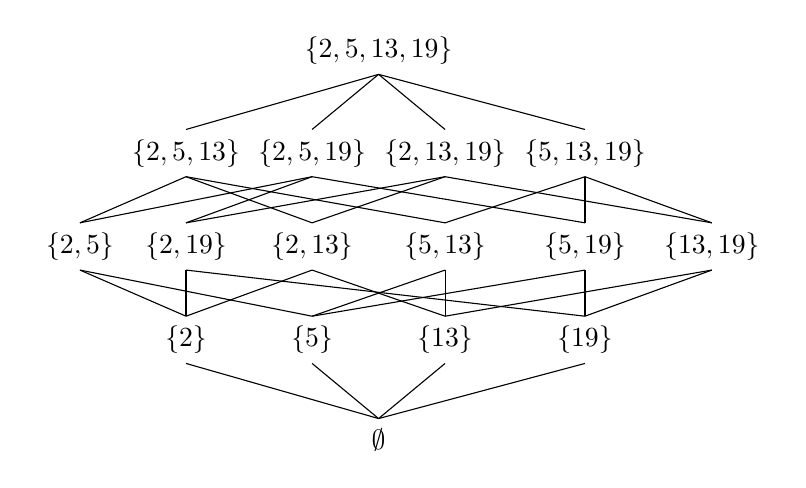
\begin{tikzpicture}
            % \hspace{-.4cm}
            \matrix (A) [matrix of nodes, row sep=.6cm, nodes={minimum width=1cm}]
            {
                \\
                & $\{2, 5, 13\}$ & $\{2, 5, 19\}$ & $\{2, 13, 19\}$ & $\{5, 13, 19\}$ &  \\
                $\{2, 5\}$ & $\{2, 19\}$ & $\{2, 13\}$ & $\{5, 13\}$ & $\{5, 19\}$ & $\{13, 19\}$ \\
                & $\{2\}$ & $\{5\}$ & $\{13\}$ & $\{19\}$ & \\
            };
            
            \node[above=1cm] at ($(A-2-3)!0.5!(A-2-4)$) (top) {$\{2, 5, 13, 19\}$};
            \foreach \i in {2,...,5}
            \draw (top.south) -- (A-2-\i.north);
            
            \foreach \i/\j in {1/1, 1/3, 1/4, 2/1, 2/2, 2/5, 3/2, 3/3, 3/6, 4/4, 4/5, 4/6}
                \pgfmathsetmacro{\i}{int(\i+1)}
                \draw (A-2-\i.south)--(A-3-\j.north);
            
            \foreach \i/\j in {1/1, 1/2, 2/1, 2/4, 3/1, 3/3, 4/2, 4/3, 5/2, 5/4, 6/3, 6/4}
            \pgfmathsetmacro{\j}{int(\j+1)}
            \draw (A-3-\i.south)--(A-4-\j.north);
            
            \node[below=1cm] at ($(A-4-3)!0.5!(A-4-4)$) (bottom) {$\emptyset$};
            \foreach \i in {2,...,5}
            \draw (A-4-\i.south)--(bottom.north);
        \end{tikzpicture}
        }
        \caption{Dependency graph of poset $(\mathcal{P}(\{2, 5, 19, 13\}), \subseteq)$.}
        \label{fig:Q2}
    \end{figure}
    
    Using the formalism of posets, we can now define the problem of computing an optimal schedule. We do so in the language of job scheduling, as it's the most common form. 

    \vspace{3mm} Assume that some task $T$ can be deocmposed into sub-tasks $T = \{T_{1}, T_{2}, \dots, T_{n}\}$. In general, we can encode the relationships between the various $T_{i}$ as a poset, where $T_{i} \prec T_{j}$ if (sub)task $T_{i}$ needs to be performed before $T_{j}$. \textbf{Assume each task $T_{i}$ takes 1 unit of time to complete.} Given $k$ processors $P_{1}$, $P_{2}$, \dots, $P_{k}$ a \textbf{schedule} for $T$ assigns each sub-task $T_{i}$ a processor $P_{j}$ as well as a time $t_{i}$ at which $P_{j}$ shoudl start task $T_{i}$. Observe that if a processor starts $T_{i}$ at times $t_{i}$, then the task will complete at time $t_{i} + w_{i}$, where $w_{i}$ is the weight of $T_{i}$. A schedule is \textbf{feasible} if:

    \begin{enumerate}[label = \arabic*]
        \item no single processor is performing multiple tasks at the same time (i.e., if a processor is assigned $T_{i}$ at time $t_{i}$ and $T_{j}$ at time $t_{j} > t_{i}$, then $t_{j} \ge t_{i} + w_{i}$), and
        \item for every pair of tasks $T_{i}$ and $T_{j}$ with $T_{i} \prec T_{j}$, $T_{j}$ is schedule to start some time after (or at the same time) $T_{i}$ completes (i.e., $t_{j} \ge t_{i} + w_{i}$).
    \end{enumerate}


    

    If we have only one processor, then the answer is fairly simple, just create a topological sorting: Definition: A topological sorting is a total ordering of a partially ordered set.

    

    \begin{algorithm}
        \caption{\textsc{topological\_sort}$(poset)$}\label{alg:cap}
        \label{alg:topological_sort}
        \begin{algorithmic}
            \State $T = $ empty list
            \State $S = $ all minimal elements in $poset$
            \While{S is not empty}
            
                remove some node $u$ from $S$ and add it to $T$.

                \State $uv\_dependencies$ set of all dependencies of the form $(u, v)$ for some $v$.
                \For{each $(u, v)$ in $uv\_dependencies$}

                    \If {v is minimal}
                        Insert v in T
                    \EndIf

                \EndFor

            \EndWhile
            
                
            \State \Return{T}
        \end{algorithmic}
    \end{algorithm}


    \vspace{3mm}
    \begin{tcolorbox}[colback=yellow!30]
        \textbf{In this part, you'll implement the following function:}
        
        \lstinline{topological_sort(poset)}: This method takes in a partially ordered set in the form of a dependency list and returns a valid topological sort. 

        I'll be manually checking that you used some semblance of Kahn's algorithm in your solution, so don't use other approaches like a modified DFS (besides, it'll be more useful for the next part).

        Tip: The use of external data structures such as queues or stacks may be helpful (but not required) in completing this task.
    \end{tcolorbox}

\section*{Part 4: Multi-Processor Job Scheduling}

    Now suppose we have multiple processors. Modify your algorithm from the last part to accomodate this change

    % https://link.springer.com/article/10.1023/B:ORDE.0000034609.99940.fb



    \subsection*{Dual Dilworth's Theorem}


    \begin{tcolorbox}[colback=yellow!40]
        \lstinline{generate_schedule(poset, num_processors)}:  This method takes in a partially ordered set in the form of a dependency list and returns a valid schedule in the form of a list of lists, where the $i$-th element in the list represents the jobs we should schedule at time $t = i$.
    \end{tcolorbox}





% \section*{(Optional) Dilworth's Theorem}
%         In the previous section, you were given infinite processors. However, this is not always the case, and there are many situations when we need to minimize the number of machines working on a certain task.

    
%         In the previous section, you devised a method to find the height of a poset. A natural question then, is how to find the \textit{width} of a poset. While this problem seems simple on the surface, it is actually much more difficult. 
        
%     \subsubsection*{Incorrect Approach}

%     using the previous section, i'm sure many of you are picturing the following approach
    
%     apply a topological sort on the DAG
%     traverse over the nodes by the topological order, calculate the minimum level:
%     no parents: 0
%     otherwise: minimum parent level + 1
%     return the max level width (max num of nodes assigned the same level).

%     However, this approach does not always work. For a salient counterexample, consider a tree.

%     also discuss how bfs wouldnt work

%     % \textbf{Note: From this point onwards, we depart from the usual land of long-estabished results, and move on to areas of ongoing research.}

%     For example, the tools used to solve these problems are used in real life for countless companies (see https://github.com/google/or-tools)


\section*{Submission Instructions (10 pts)}
    After you fill the appropriate functions, submit the following files to Gradescope and make sure you pass all test cases:
    \begin{itemize}
        \item \lstinline{relations.py}
        \item \lstinline{scheduler.py}
    \end{itemize}

    \vspace{3mm}
    \textbf{Notes}

    \begin{itemize}
        \item The autograder may not reflect your final grade on the assignment. We reserve the right to run additional tests during grading.
        \item Do not import additional packages, as your submission may not pass the test cases or manual review.
    \end{itemize}

    

\end{document}